%
% The Quantum Ecosystem
%

\section{The quantum ecosystem}\index{Ecosystems}

\famousquote{The most dangerous worldview is the worldview of those who have not viewed the world.}{Alexander von Humboldt}
\newline

\dropcap{A}{ssociated} with any new computer platform comes a hardware/software \textit{ecosystem}\index{Ecosystems} that evolves around it. If we consider the release of the original iPhone\index{iPhone} and its iOS\index{iOS} operating system, it wasn't just the product itself that was revolutionary, but the third-party software industry that emerged surrounding it, and it wasn't until this software ecosystem emerged on the App Store\index{App Store} that the product realised its full potential and became truly transformative.

From the hardware perspective, it wasn't until interfacing standards such as USB\index{USB} and Wi-Fi\index{Wi-Fi} emerged, allowing the plethora of competing hardware products to arbitrarily interconnect and interface with one another, that the hardware realised its full potential.

In the quantum era we anticipate the same phenomena to arise. What will this \textit{quantum ecosystem} look like? Here are some of the elements that vendors might specialise in, providing compatible components for the quantum ecosystem:

\begin{itemize}
\item Quantum operations: vendors selling the capacity for non-trivial state preparation (e.g Bell, NOON\index{NOON states} and GHZ\index{GHZ states} states), or measurements (e.g complex entangling syndrome measurements\index{Syndrome measurements}).

\item Software subroutines:\index{Subroutines} Much like classical code, many quantum computations (and other quantum protocols) can be decomposed into pipelines of subroutines. There are many quantum operations that arise repeatedly (such as quantum Fourier transforms and syndrome calculations), which vendors might specialise in for outsourcing.

\item Oracles:\index{Oracles} As an essential quantum software building block, oracles will become a fundamental unit for outsourcing. These oracles will store hard-corded or algorithmically-generated databases, or mathematical functions. For example, for use in genetic medicine (Sec.~\ref{sec:genetic_medicine}), such databases could algorithmically generate tables of candidate drug compounds, or they could implement mathematical functions whose input space is to be searched over when quantum-enhancing the solving of \textbf{NP}-complete\index{NP and NP-complete} problems.

\item Interfacing:\index{Interfacing} \textit{De facto} standards will emerge for interconnecting quantum hardware units. Most notably, standards for optical interconnects will arise.

\item Modularisation:\index{Modularisation} Arbitrarily-interconnectable units will develop, allowing quantum hardware to be constructed in an ad hoc, Lego-like\index{Lego} manner. These modules could implement small elements of a larger quantum computation, such as housing a small part of a larger graph state (Sec.~\ref{sec:module}), communications building blocks (such as transmitters or receivers of Bell pairs), or algorithmic building blocks such as quantum Fourier transforms (Sec.~\ref{sec:QFT_alg}).

\item Classical pre-, post- or intermediate-processing:\index{Classical processing} Quantum computation, and other quantum protocols, typically require some degree of classical pre- or post-processing, or feedforward. These classical operations can be highly non-trivial. For example, a novel topological quantum error correcting code\index{Quantum error correction} (Sec.~\ref{sec:surface_codes}) might require complex encoding, decoding and feedforward operations. Determining and implementing these operations may require complicated optimisation protocols. These might be outsourced to a specialised provider.

\item Classical control:\index{Classical control} Many quantum protocols require intermediate classical control, for example for feedforward\index{Feedforward}. For example, in a quantum repeater network we must control the order of entangling operations and track local Pauli corrections accumulated by the final entangled Bell pair.

\item Quantum memory:\index{Quantum memory} Storing qubits with long decoherence lifetimes is extremely challenging using today's technology, and it is foreseeable that vendors might specialise in this particular operation, especially once error correction is built into the memory. 

\item Quantum error correction:\index{Quantum error correction} Any given quantum error correcting code follows a well-defined recipe for encoding, correction, and decoding. Thus, it might become an example of a subroutine specialised in by a dedicated quantum error correction vendor, and licensed out as a building block for embedding into larger, fault-tolerant\index{Fault-tolerance} protocols.

\item Time-share licensing market:\index{Time-share licensing market} A market will emerge for the trade and allocation of time-shares on the global virtual quantum computer (Sec.~\ref{sec:glob_unif_quant_cloud}). Associated financial services industries\index{Financial services industries} will emerge around this marketplace, including secondary markets\index{Secondary markets}, derivative markets\index{Derivative markets}, managed funds in quantum infrastructure\index{Managed funds}, and IPO markets\index{Initial public offering (IPO) markets}.
\end{itemize}

A map of just a few of the potential hardware and software elements to emerge in the quantum ecosystem is presented in Fig.~\ref{fig:ecosystem}.

\begin{figure}[!htpb]
\if 2\pubmode
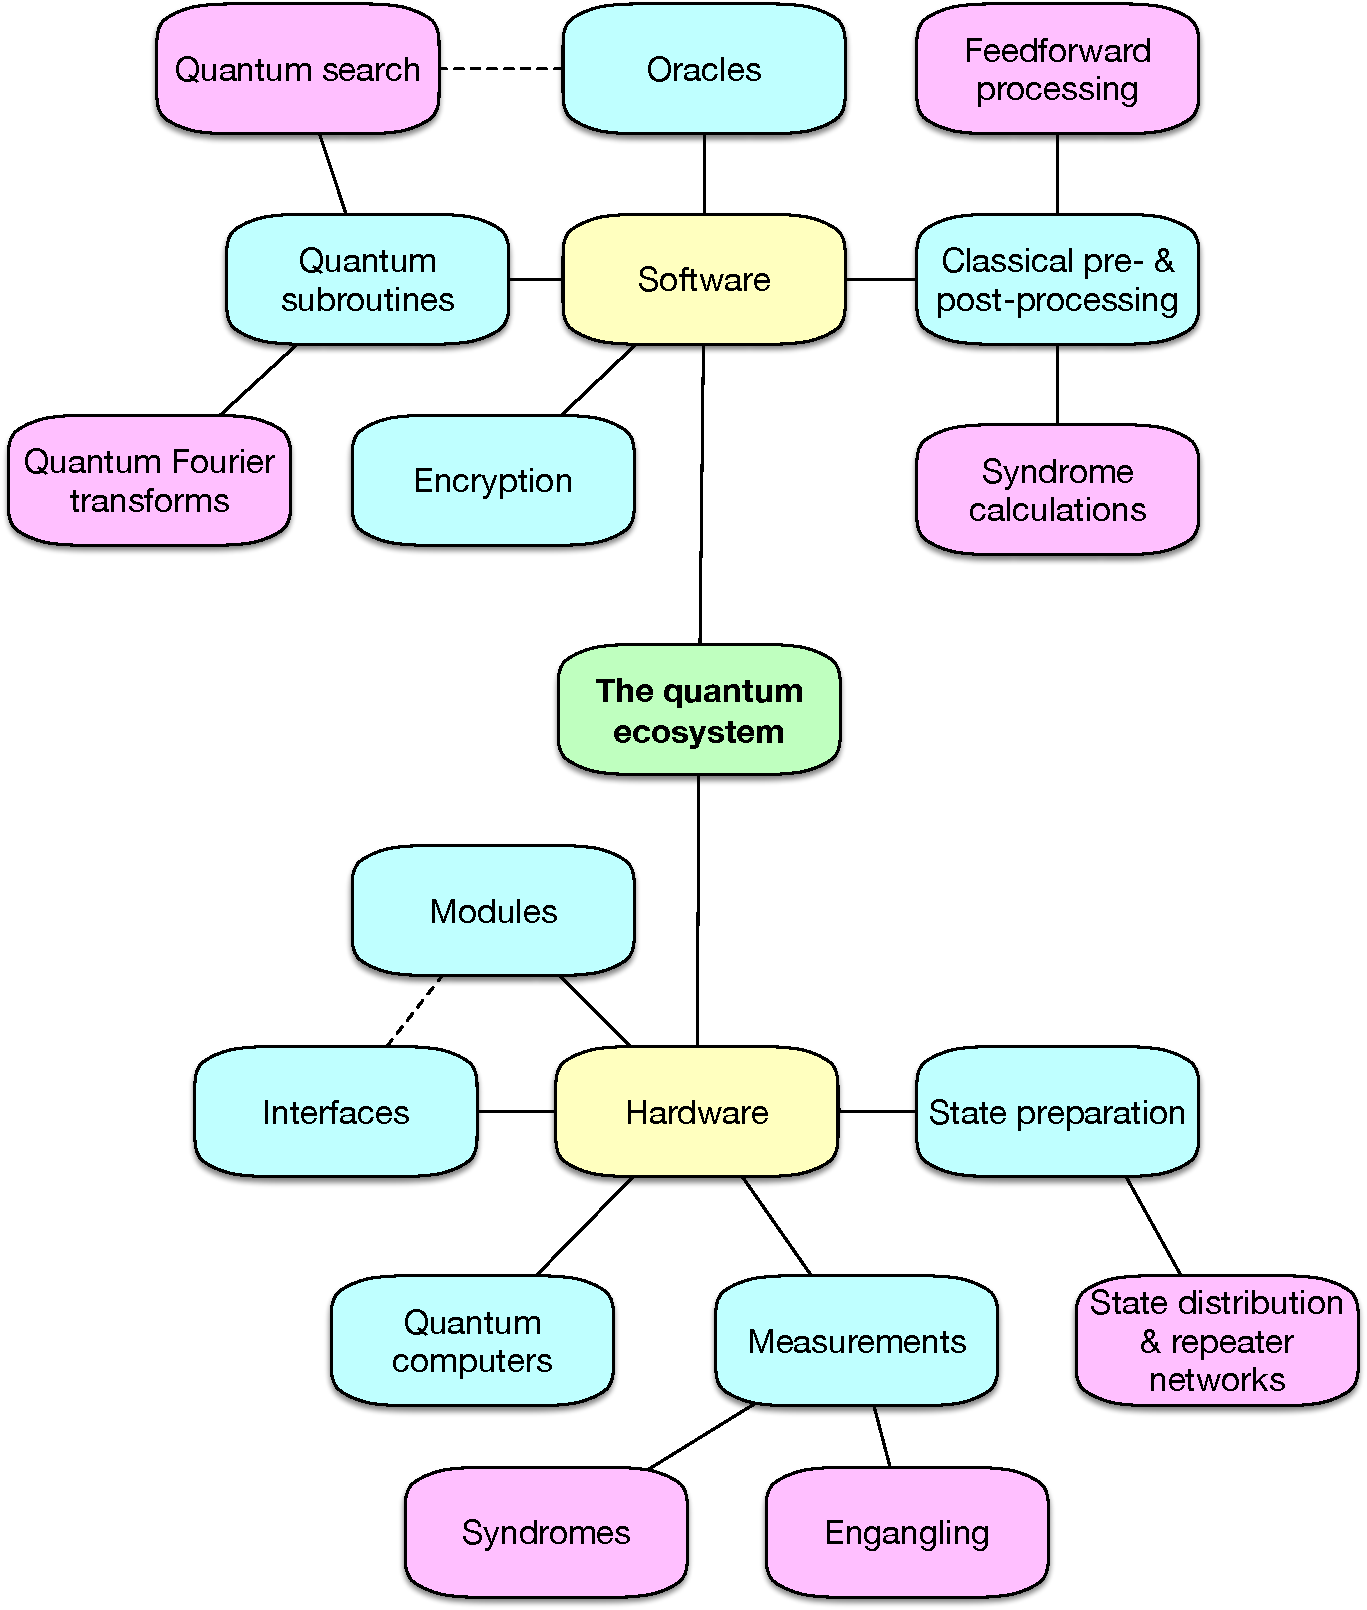
\includegraphics[clip=true, width=0.475\textwidth]{ecosystem_long}
\else
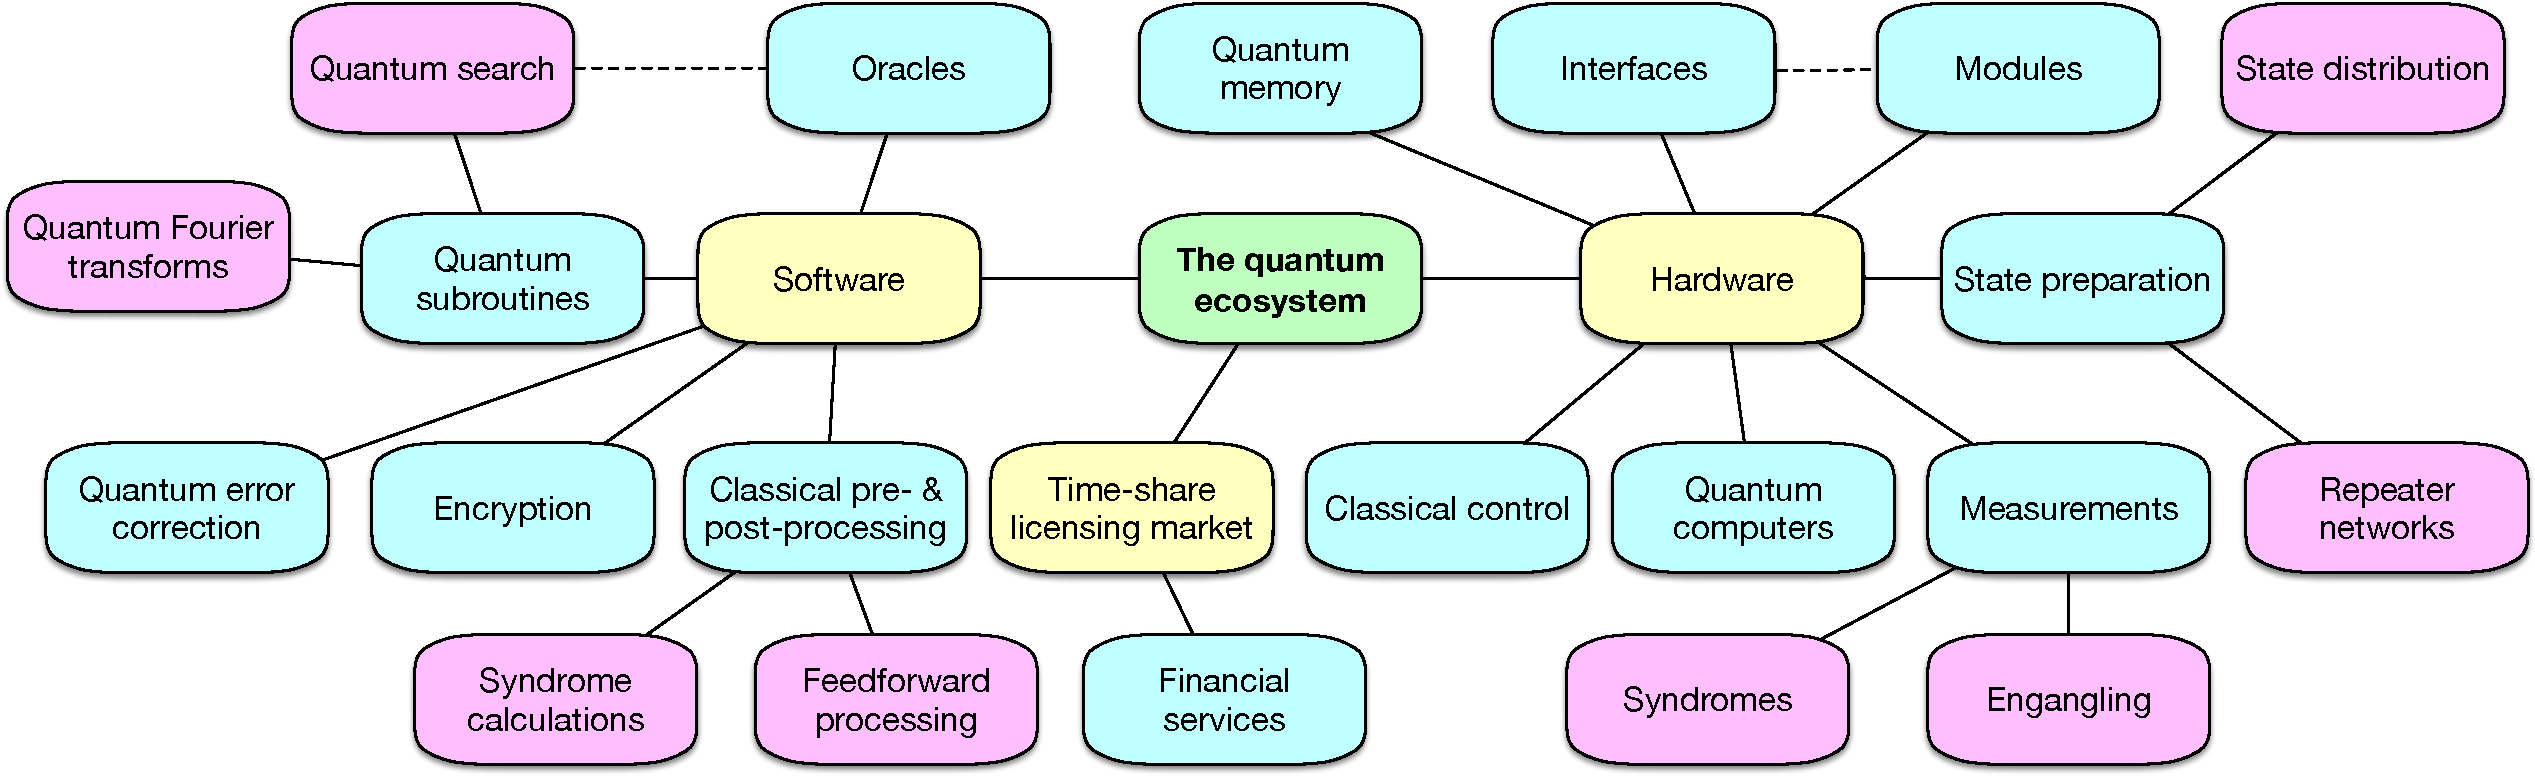
\includegraphics[clip=true, width=\textwidth]{ecosystem}
\fi
\caption{Map of just a few of the elements of the quantum ecosystem that are likely to arise with the advent of the quantum internet. The distinct units could become areas of specialisation for quantum vendors, which might be licensed out or sold to customers as discrete units, or as complete integrated processing pipelines, all outsourced and distributed over the quantum network.}\label{fig:ecosystem}\index{Ecosystems}	
\end{figure}